\documentclass{article}
\usepackage[T1]{fontenc}
\usepackage{lmodern}
\usepackage{graphicx}
\usepackage{amsmath,amssymb}
\usepackage[a4paper,margin=2cm]{geometry}
\usepackage[absolute,overlay]{textpos}
\setlength{\TPHorizModule}{1mm}
\setlength{\TPVertModule}{1mm}
\usepackage[indonesian]{babel}
\usepackage{hyperref}
\setlength{\emergencystretch}{2em}
% unit: Halaman 41

\begin{document}

% === Halaman 41 (llm) ===

\vspace{240.57mm}

\begin{itemize}
  \item Demo Vigenere Cipher online: \url{https://cryptii.com/pipes/vigenere-cipher}
\end{itemize}
\vspace{10mm}

% deskripsi: Screenshot antarmuka web Cryptii yang menunjukkan proses enkripsi teks menggunakan Vigenère cipher, dengan plaintext 'Betapa ramainya acara pertandingan sepakbola di lapangan itu Inginku ke sana, apadaya tidak punya karcis' dan kunci 'tabahkanhatimu', menghasilkan ciphertext yang terenkripsi.
% bbox normalisasi: [0.0600, 0.1300, 0.9300, 0.9400]
\begin{textblock*}{182.70mm}(12.60mm,38.61mm)
\noindent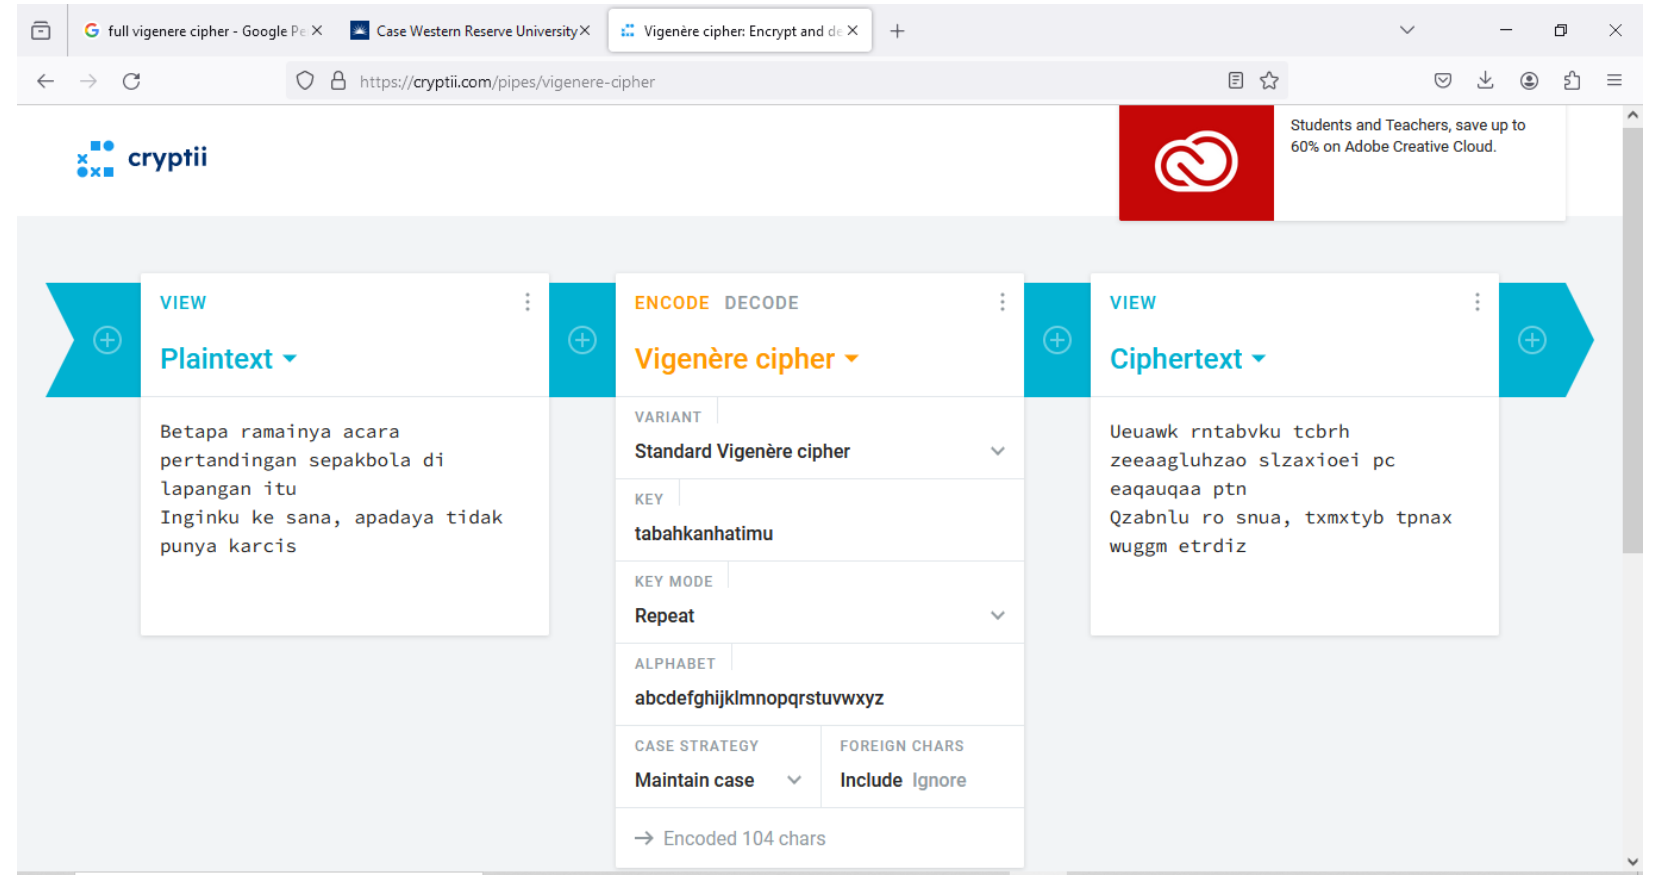
\includegraphics[width=182.70mm,height=240.57mm]{../../images/llm/page_041_img_01.png}%
\end{textblock*}

\end{document}
